\documentclass[12pt]{article}
\usepackage[utf8]{inputenc}
\usepackage{amsmath}
\usepackage{multicol}
\usepackage{graphicx}
\usepackage{float}
\usepackage{dsfont}
\usepackage{textcomp}
\usepackage{amsfonts}
\usepackage{hyperref}
\usepackage{amsmath}
\usepackage{csquotes}
\hypersetup{
    colorlinks,
    citecolor=black,
    filecolor=black,
    linkcolor=black,
    urlcolor=black
}
\usepackage{cleveref}
\usepackage{fancyhdr}
\setlength{\headheight}{14.5pt}
\renewcommand{\sectionmark}[1]{\markright{#1}{}}
\usepackage[T1]{fontenc}
\usepackage[colorinlistoftodos]{todonotes}
\usepackage[margin=2cm,a4paper]{geometry}
\newgeometry{left=2.0cm,right=2.0cm,top=2.5cm,bottom=2.5cm}
\usepackage{listings}
\setlength{\marginparwidth}{2cm}
\setlength{\parindent}{0pt}
\newcommand{\deriv}{\mathrm{d}}
\title{}
\pagestyle{fancy}
\fancyhf{}
\rhead{Section \thesection}
\lhead{Assignment 3: Photometry}
\lfoot{PH512: Data Analysis Techniques in Astronomy and Planetary Science}
\rfoot{Page \thepage}
\renewcommand{\headrulewidth}{1pt}
\renewcommand{\footrulewidth}{1pt}
\begin{document}
\begin{titlepage}
\newgeometry{left=1.0in,right=1.0in,top=0.8in,bottom=0.8in}
\newcommand{\HRule}{\rule{\linewidth}{0.5mm}}
\begin{centering} 

%---------------------------------------------------------------------------
%	TITLE SECTION
%---------------------------------------------------------------------------

\includegraphics[scale=0.7]{Images/Uni_of_Kent.png}\\[0.3cm]
\HRule \\ [0.3cm]
\Huge{\bfseries{Photometry}} \\
\textsc{\large Data Analysis Techniques in Astronomy and Planetary Science}\\ [-0.1cm]
\textsc{\large BSc(Hons) Astronomy, Space Science and Astrophysics}\\ [-0.2cm]
\HRule \\[0.5cm]
%---------------------------------------------------------------------------
\begin{minipage}{0.625\textwidth}
\begin{center} \large
{\large Author: Lukasz R Tomaszewski (lrgt2)} \\[0.2cm]
{\large Date: $12^{th}$ Feb - $4^{th}$ Mar 2020}\\[0.2cm]
{\large PH512 Assignment 3} \\[0.2cm]
{\large Word Count: 1412} \\
\end{center}
\end{minipage}\\[1cm]
\end{centering} 
\begin{tableofcontents}
\end{tableofcontents}
\end{titlepage}
\newpage
%---------------------------------------------------------------------------
%	SECTION 1
%---------------------------------------------------------------------------
\section{Photometry Analysis}
\label{Section 1}

Photometry is a measurement system used by astronomers in image processing, in particular the measurement of a celestial objects brightness over time utilizing the star magnitude index where the higher the number, the fainter the star looks to a naked eye and the lower the number, the brighter it looks to the naked eye (\cite{ImageProcessing}). Such measurements can help determine the temperature of the star that can assist in finding out the stars distance, size and density (\cite{Photometry}).  \\

Photometry works by capturing the light flux of the individual pixels of a star and then measuring and subtracting the sky background light flux that is emitted from the star, from the light flux to give the total flux light the star emits, this flux can then be converted into a magnitude. As atmospheric extinction i.e gas, clouds, exists between the camera and the target object, its sometimes necessary to select comparison stars and thus calculate the differential magnitude that can tell the exact magnitude of the star if extinctions does exist between. 


%---------------------------------------------------------------------------
%	SECTION 2
%---------------------------------------------------------------------------
\section{Single Photometry Method}
\label{Section 2}
%---------------------------------------------------------------------------
\subsection{Single-Star Photometry}
\label{SubSection 2a}


Single-Star photometry is used to determine a stars brightness by measuring the total light emitted from the star and then subtracting the light of the background sky. By selecting the "M82-x20.fts" from the AIP4WIN tutorial packet, which is a stack of 20 infrared images of the Messier 82 galaxy with a 60 second exposure (\cite{ImageProcessingTutorial}). Utilizing the 'single star' photometry tool, 4 stars were selected as shown in \cref{SS-Aperture}, upon each star is an aperture radius which is changed in size to encapsulate all the light in the star. Following the aperture radius is two annuli, where the inner annulus measures the light emitted from the star into the sky background and the outer annulus measures the sky background surrounding the selected star. The inner and outer annuli will then be subtracted as sky background against the light inside the aperture radius. \\

\begin{figure}[H]
\centering
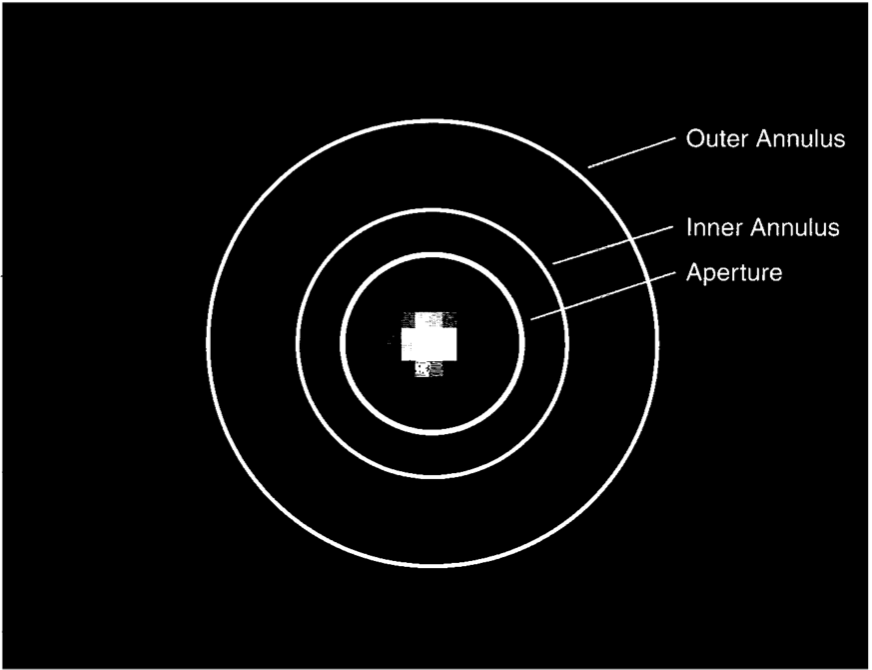
\includegraphics[scale=0.5]{Images/AsImages/Photometry.png} \\ [0.3cm]
\caption{Illustration of the aperture radius, inner and outer annulus and their suitable distance from the star}
\label{SS-Annuli}
\end{figure}

\begin{figure}[H]
\centering
\begin{multicols}{2}
\begin{minipage}[H]{0.5\textwidth}
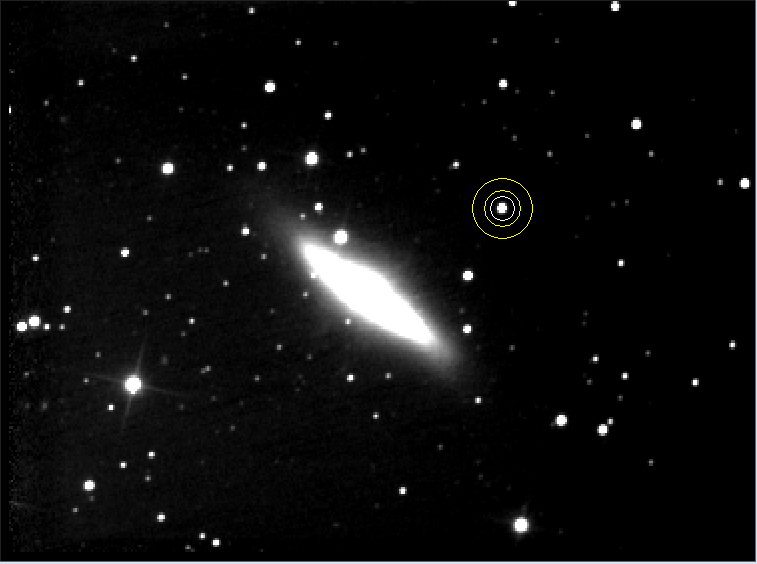
\includegraphics[scale=0.43]{Images/AsImages/SS/Sr1-Aperture.PNG} \\
\end{minipage}
\begin{minipage}[H]{0.5\textwidth}
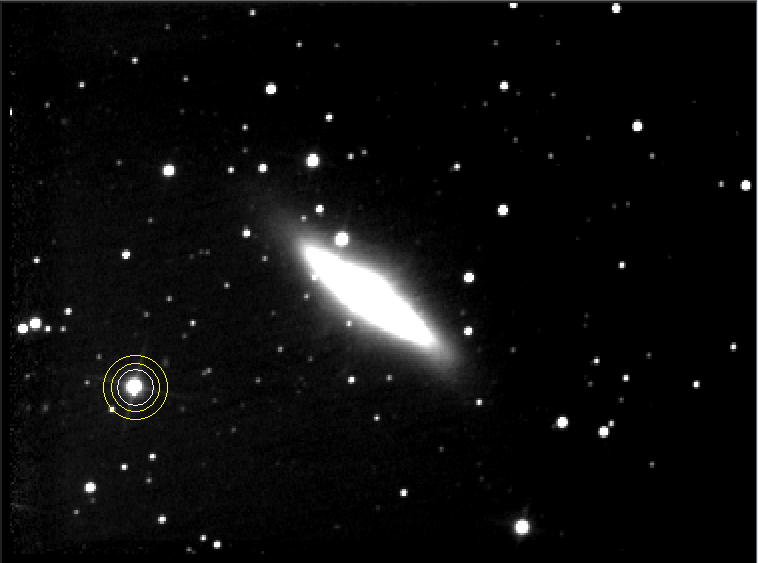
\includegraphics[scale=0.43]{Images/AsImages/SS/Sr3-Aperture.PNG}
\end{minipage}
\begin{minipage}[H]{0.5\textwidth}
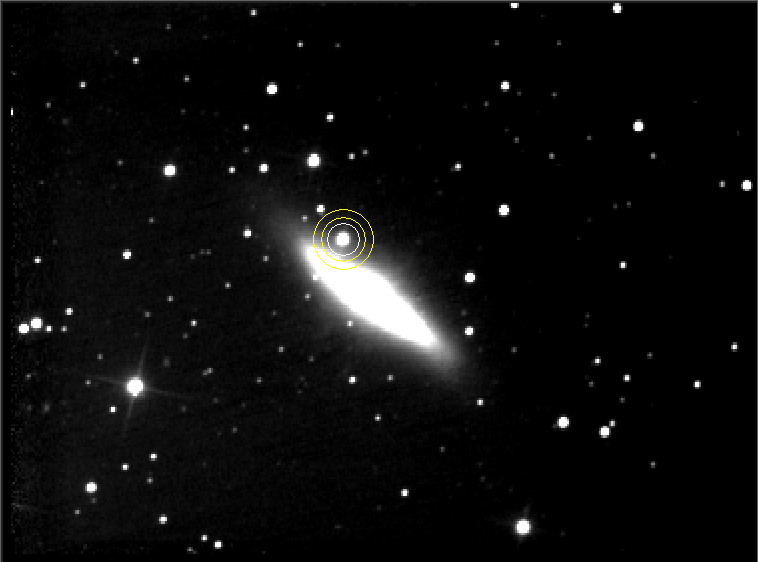
\includegraphics[scale=0.43]{Images/AsImages/SS/Sr2-Aperture.PNG} \\
\end{minipage}
\begin{minipage}[H]{0.5\textwidth}
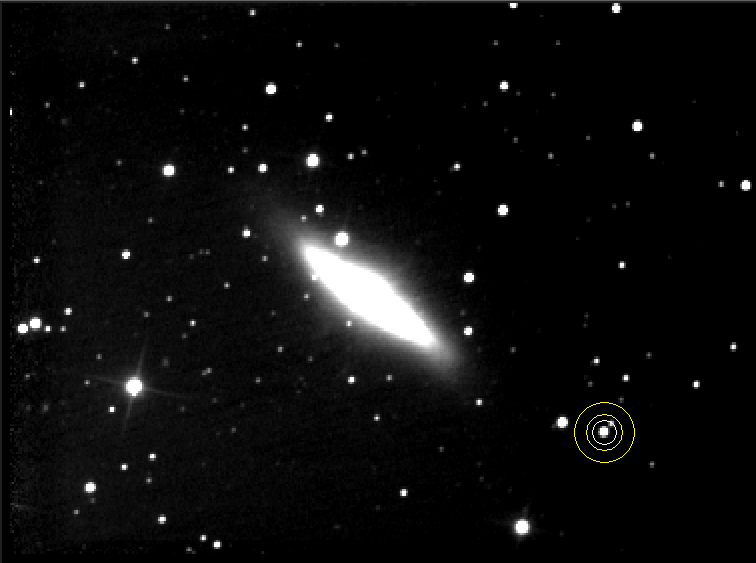
\includegraphics[scale=0.43]{Images/AsImages/SS/Sr4-Aperture.PNG}
\end{minipage}
\end{multicols}
\caption{AIP4WIN image of the Messier 82 galaxy with the photometry tool 'Single-Star' depicting the aperture, inner and outer anuli around each target star for photometric measurements of four stars surrounding the galaxy. Star 1 = top right, Star 2 = top right, Star 3 = bottom left and Star 4 = bottom right.}
\label{SS-Aperture}
\end{figure}

\begin{table}[H]
\begin{center}
 \footnotesize
 \begin{tabular}{|c||c|c|c||c||c|c|}
 \hline
 \multicolumn{7}{|c|}{AIP4WIN Photometry settings for all four target single-star images} \\
 \hline \hline
 Target & Aperture & Inner Annulus & Outer Annulus & Sky Annulus & Integration & Zero  \\
 Star & Radius & Radius & Radius & Pixels & Time (s) & Point \\
 \hline \hline
 S1 & 6.0 & 9.0 & 15.0 & 236 & 60 & 25 \\
 \hline
 S2 & 6.0 & 11.0 & 15.0 & 171 & 60 & 25 \\
 \hline
 S3 & 9.0 & 11.0 & 16.0 & 179 & 60 & 25 \\
 \hline
 S4 & 6.0 & 9.0 & 15.0 & 100 & 60 & 25  \\
 \hline
 \end{tabular} \\ [0.5cm]
 \begin{tabular}{|c||c|c||c|c|c||c|c|}
 \hline
 \multicolumn{8}{|c|}{Photometric data collected of the four target single-star images} \\
 \hline \hline
 Target Star & Star$_X$ & Star$_Y$ & ADU$_{Max}$ & ADU$_{Sky}$ & ADU$_{Star}$ & Magnitude & Sigma\\
 \hline \hline
 S1 & 249.999 & 88.579 & 2028.0 & 180.8136 & 15,567.9 & 18.965 & $\pm$0.016 \\
 \hline
 S2 & 169.516 & 101.010 & 3904.0 & 327.854 & 36,924.9 & 18.027 & $\pm$0.010 \\
 \hline
 S3 & 65.778 & 164.720 & 4086.0 & 223.56 & 17,624.0 & 17.308 & $\pm$0.007 \\
 \hline
 S4 & 300.405 & 183.969 & 2009.0 & 175.8789 & 16,458.02 & 18.904 & $\pm$0.016 \\
 \hline
 \end{tabular} \\ 
 \caption{AIP4WIN settings and photometry data of the 4 target 'single-star' stars.}
 \label{SS Data}
\end{center}
\end{table} 

\begin{figure}[H]
\centering
\begin{multicols}{2}
\begin{minipage}[H]{0.5\textwidth}
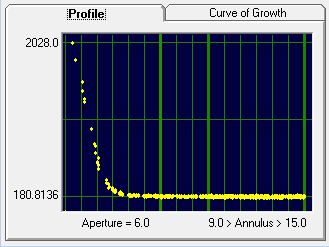
\includegraphics[scale=1.0]{Images/AsImages/SS/Sr1-Profile.PNG} \\
\end{minipage}
\begin{minipage}[H]{0.5\textwidth}
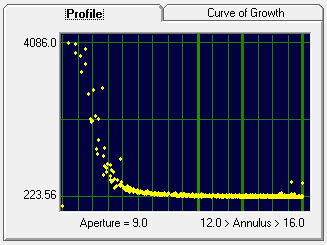
\includegraphics[scale=1.0]{Images/AsImages/SS/Sr3-Profile.PNG}
\end{minipage}
\begin{minipage}[H]{0.5\textwidth}
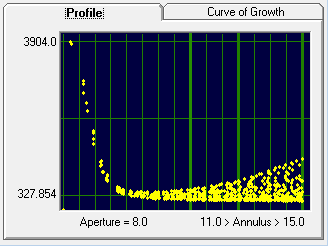
\includegraphics[scale=1.0]{Images/AsImages/SS/Sr2-Profile.PNG} \\
\end{minipage}
\begin{minipage}[H]{0.5\textwidth}
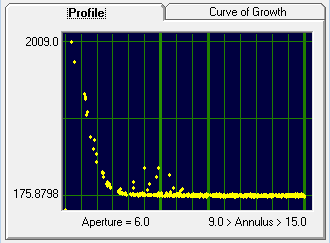
\includegraphics[scale=1.0]{Images/AsImages/SS/Sr4-Profile.PNG}
\end{minipage}
\end{multicols}
\caption{AIP4WIN image of the Messier 82 galaxy with the photometry tool 'Single-Star' depicting the photometric profile of four stars surrounding the galaxy. Star 1 = top right, Star 2 = top right, Star 3 = bottom left and Star 4 = bottom right.}
\label{SS-Profile}
\end{figure}

The profile of a star is its brightness over a cross-section, where the individual pixel values of light are plotted against the distance from the centre of the star in reference to the annulus, as they decline gradually it shows a perfect light profile, where the inner annulus of star 2 encases a separate star, the light profile has a spray effect nearer to the annulus. \\

\begin{figure}[H]
\centering
\begin{multicols}{2}
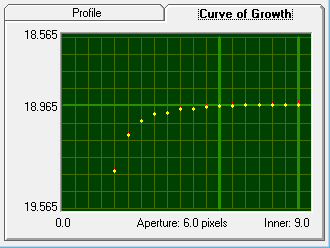
\includegraphics[scale=1.0]{Images/AsImages/SS/Sr1-Growth.PNG} \\ [0.2cm]
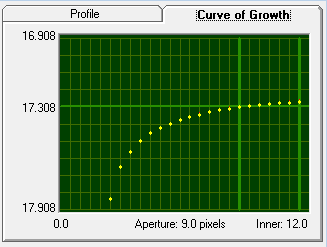
\includegraphics[scale=1.0]{Images/AsImages/SS/Sr3-Growth.PNG}
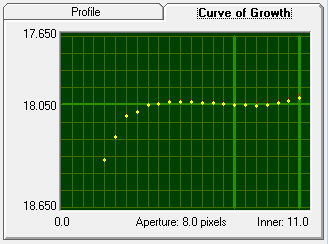
\includegraphics[scale=1.0]{Images/AsImages/SS/Sr2-Growth.PNG} \\ [0.2cm]
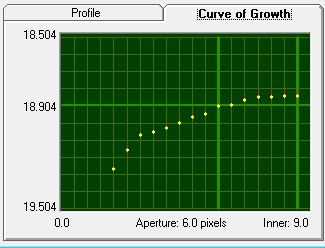
\includegraphics[scale=1.0]{Images/AsImages/SS/Sr4-Growth.PNG}
\end{multicols}
\caption{AIP4WIN image of the Messier 82 galaxy with the photometry tool 'Single-Star' depicting the photometric curves of growth of four stars surrounding the galaxy. Star 1 = top right, Star 2 = top right, Star 3 = bottom left and Star 4 = bottom right.}
\label{SS-Growth}
\end{figure}

The curve of growth of a star is used to determine a good aperture radius of the star so that it captures all the emitted light, where the graph plots the stars magnitude against the aperture radius. The level regions in stars 1,2 and 3 in \cref{SS-Growth} shows that the aperture radius is slightly small as the plot doesn't fall near the inner annulus so the it would need to be increased whereas for star 4, the aperture radius is too big that its borders the edge of the M82 galaxy and thus the light emitted from the galaxy itself has disrupted the data. 

%---------------------------------------------------------------------------
\subsection{Single-Image Photometry}
\label{SubSection 2b}

Single-Image photometry is used to calculate the magnitudes of two or more stars and thus also the difference in magnitude of all measured stars. It also measures the light and automatically subtracts the background sky light from it, by selecting comparison stars allows for more accurate measurements to be recorded as atmospheric extinction may cause a incorrect measurement of a stars light flux  (\cite{ImageProcessingTutorial}). \\

\begin{figure}[H]
\centering
\begin{multicols}{2}
\begin{minipage}[H]{0.5\textwidth}
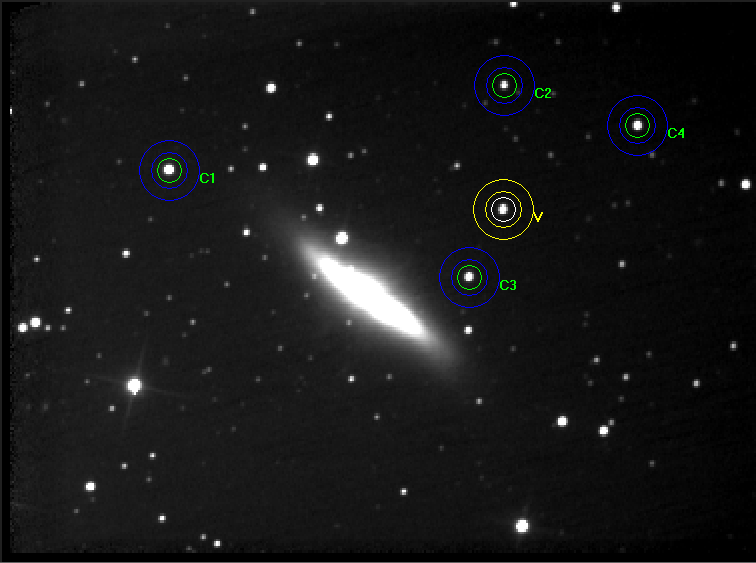
\includegraphics[scale=0.43]{Images/AsImages/SI/Sr1-Aperture.PNG} \\ 
\end{minipage}
\begin{minipage}[H]{0.5\textwidth}
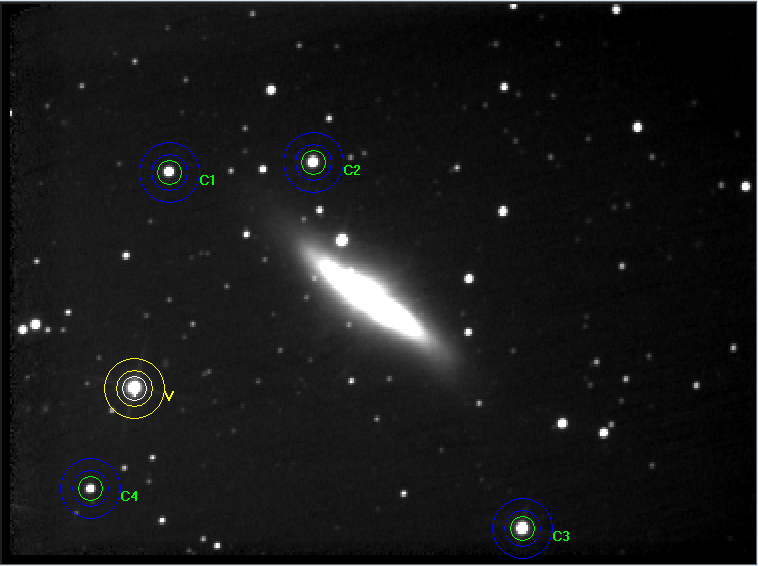
\includegraphics[scale=0.43]{Images/AsImages/SI/Sr3-Aperture.PNG}
\end{minipage}
\begin{minipage}[H]{0.5\textwidth}
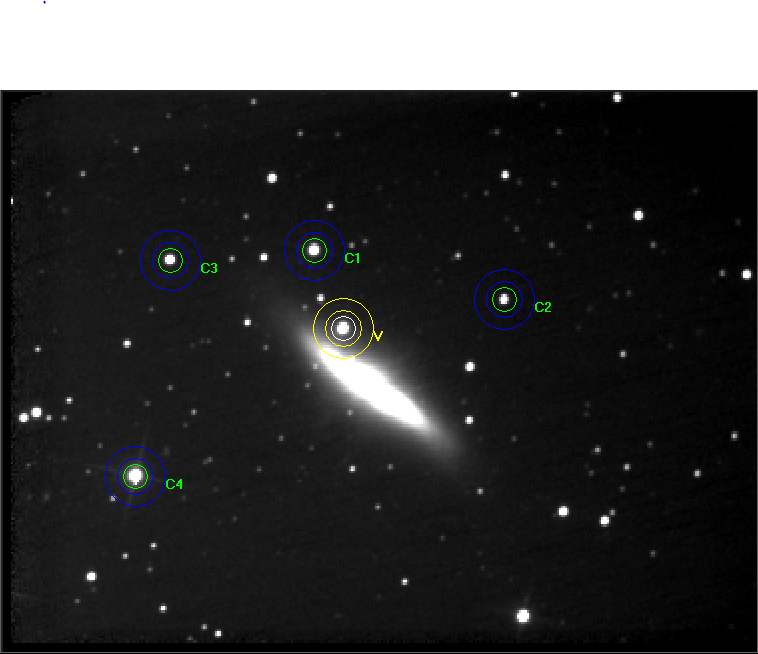
\includegraphics[scale=0.43]{Images/AsImages/SI/Sr2-Aperture.PNG} \\ 
\end{minipage}
\begin{minipage}[H]{0.5\textwidth}
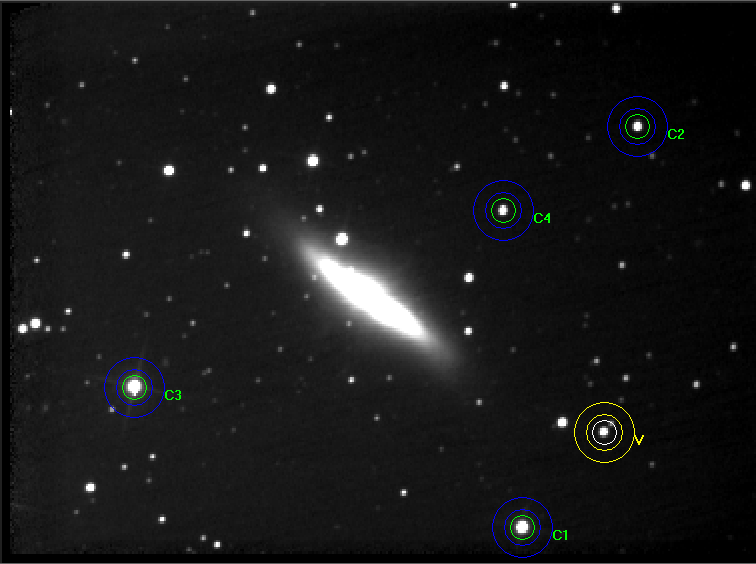
\includegraphics[scale=0.43]{Images/AsImages/SI/Sr4-Aperture.PNG}
\end{minipage}
\end{multicols}
\caption{AIP4WIN image of the Messier 82 galaxy with the photometry tool 'Single-Image' depicting the aperture, inner and outer anuli around each target star with 4 comparison stars for each target star for photometric measurements of four stars surrounding the galaxy. Star 1 = top right, Star 2 = top right, Star 3 = bottom left and Star 4 = bottom right.}
\label{SI-Aperture}
\end{figure}

Utilizing the single image tool, the target star is chosen and a number of comparison stars are selected to which the magnitude will be display as the comparison star/s are brighter or dimmer than the target star as displayed in \cref{SI-Aperture} which the resulting magnitudes are displayed in \cref{SI Data}. \cref{SI Data} also displays the differential magnitude of the target star minus a comparison star so that they can be compared to decipher is the target star is undergoing any atmospheric extinction. \\ 

\begin{table}[H]
\begin{center}
 \footnotesize
 \begin{tabular}{|c||c|c|c||c||c|c|}
 \hline
 \multicolumn{7}{|c|}{AIP4WIN Photometry settings for all four target single-image images} \\
 \hline \hline
 Target & Aperture & Inner Annulus & Outer Annulus & Sky Annulus & Integration & Zero  \\
 Star & Radius & Radius & Radius & Pixels & Time (s) & Point \\
 \hline \hline
 S1 & 6.0 & 9.0 & 15.0 & 236 & 60 & 25 \\
 \hline
 S2 & 6.0 & 9.0 & 15.0 & 232 & 60 & 25 \\
 \hline
 S3 & 6.0 & 9.0 & 15.0 & 235 & 60 & 25 \\
 \hline
 S4 & 6.0 & 9.0 & 15.0 & 100 & 60 & 25  \\
 \hline
 \end{tabular} \\ [0.5cm]
 \begin{tabular}{|c|c||c|c||c|c|c||c|c|}
 \hline
 \multicolumn{9}{|c|}{Photometric data collected of the four target single-image images} \\
 \hline \hline
 Star & Target & Star$_X$ & Star$_Y$ & ADU$_{Max}$ & ADU$_{Sky}$ & ADU$_{Star}$ & Magnitude & Sigma\\
 \hline \hline
 1& Var & 249.999  & 88.579&     2028.0       &    180.8136    &15567.9   &18.965 &$\pm$0.0162 \\
 1&  C1 &  83.037   &71.512   &  3072.0         &     203.88  & 26140.66   &18.402 &$\pm$0.0108 \\
 1&  C2  &250.566   &35.092   &  1247.0         &   164.0773 &  8381.197  & 19.637 &$\pm$0.0280\\
 1&  C3  &232.987  &117.565    & 2065.0          &    195.9958 &  15285.41  & 18.985 & $\pm$0.0167\\
 1&  C4  &317.147   &52.471     &1817.0          & 154.9872  & 15789.23  & 18.949& $\pm$ 0.0154\\
  1&  Ens  &    &      & & 179.7343  & 65542.64  & 17.404 & $\pm$ 0.0078\\
 \hline \hline
 2& Var & 169.516 & 101.010  &   3904.0   &    322.263  & 37495.18 &  18.010 &0.0091\\
 2&  C1 & 155.045 &  67.267   &  3569.0   & 199.406  & 33323.62   &18.139 &0.0089\\
 2&  C2  &249.999  & 88.579    & 2028.0    & 180.8136 &   15567.9  & 18.965& 0.0162\\
 2&  C3   &83.037  & 71.512     &3072.0      &  203.88  & 26140.66   &18.402& 0.0108\\
 2&  C4   &65.746  &164.741     &4086.0      & 228.596  & 66354.21   &17.391& 0.0055\\
   2&  Ens  &    &      &  & 203.153  & 141417  & 116.569 & $\pm$ 0.0043\\
 \hline \hline
 3& Var &  65.746  &164.741   &  4086.0  &  228.596 &  66354.21 &  17.391& 0.0055 \\
 3&  C1  & 83.037   &71.512     &3072.0  &203.88  & 26140.66   &18.402 &0.0108\\
 3&  C2  &155.045   &67.267    & 3569.0   & 199.406 &  33323.62 &  18.139 &0.0089\\
 3&  C3  &259.623  &225.015   &  3953.0   &186.1348  & 48049.52  & 17.741& 0.0068\\
 3&  C4   &43.718  &207.962     &2561.0     & 215.597   &16862.34  & 18.878& 0.0161\\
   3&  Ens  &    &      &  & 201.301  & 124355.4  & 16.709 & $\pm$ 0.0047\\
 \hline \hline
 4&  Var & 300.405  &183.969   &  2009.0    & 175.8798  & 16458.02 &  18.904 &0.0156 \\
 4&  C1 & 259.623 & 225.015    & 3953.0   & 186.1348  & 48049.52  & 17.741& 0.0068\\
 4&  C2  &317.147  & 52.471  & 1817.0   &154.9872  & 15789.23 &  18.949 & 0.0154\\
 4&  C3   &65.746  &164.741   & 4086.0   & 228.596  & 66354.21 &  17.391 & 0.0055\\
 4&  C4  &249.999  & 88.579  & 2028.0 & 180.8136   & 15567.9  & 18.965& 0.0162\\
   4&  Ens  &    &      & & 187.6335  & 145795.5  & 16.536 & $\pm$ 0.0041\\
 \hline 
 \end{tabular} \\[0.5cm]
 \begin{tabular}{|c||c|c|c|}
 \hline
 \multicolumn{4}{|c|}{Magnitudes for all four target single-image images} \\
 \hline 
 Star & (V-C1) \& Sigma & (C2-C1) \& Sigma & (V-Ens) \& Sigma\\
 \hline \hline
 1 & 0.563 $\pm$ 0.0195 &  1.235 $\pm$ 0.0300 &  1.561 $\pm$ 0.0179 \\
 \hline
 2 & -0.128 $\pm$ 0.0128 &  0.826 $\pm$ 0.0184 &  1.441 $\pm$ 0.0101 \\
 \hline
 3 & -1.011 $\pm$ 0.0121 &  -0.264 $\pm$ 0.0140 &  0.682 $\pm$ 0.0072 \\
 \hline
 4 & 1.163 $\pm$ 0.0170 &  1.208 $\pm$ 0.0169 &  2.368 $\pm$ 0.0162 \\
 \hline
 \end{tabular} \\
 \caption{AIP4WIN settings and photometry data of the 4 target 'single-image' stars.}
 \label{SI Data}
\end{center}
\end{table} 

\begin{figure}[H]
\centering
\begin{multicols}{2}
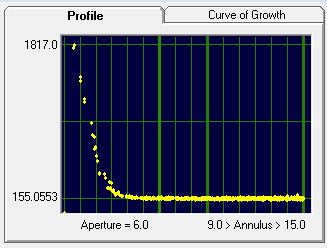
\includegraphics[scale=1.0]{Images/AsImages/SI/Sr1-Profile.PNG} \\ [0.2cm]
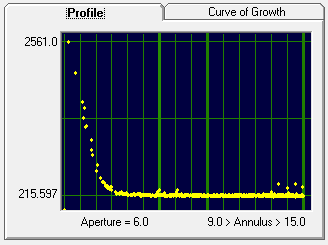
\includegraphics[scale=1.0]{Images/AsImages/SI/Sr3-Profile.PNG}
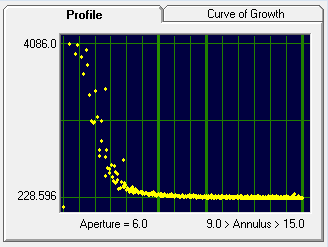
\includegraphics[scale=1.0]{Images/AsImages/SI/Sr2-Profile.PNG} \\ [0.2cm]
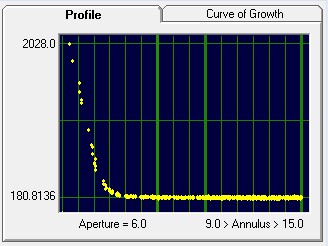
\includegraphics[scale=1.0]{Images/AsImages/SI/Sr4-Profile.PNG}
\end{multicols}
\caption{AIP4WIN image of the Messier 82 galaxy with the photometry tool 'Single-Image' depicting the photometric profile of four stars surrounding the galaxy. Star 1 = top right, Star 2 = top right, Star 3 = bottom left and Star 4 = bottom right.}
\label{SI-Profile}
\end{figure}

The profiles in \cref{SI-Profile} show all the target star light flux profile over a cross section, it also shows no interference from any other stars. Below in \cref{SI-Growth} it confirms this apart from star 2 where the inner annulus sits over a nearby star causing the curve of growth to deviate upwards instead of leveling out, to fix this error would be to make the inner annulus smaller. \\ 

\begin{figure}[H]
\centering
\begin{multicols}{2}
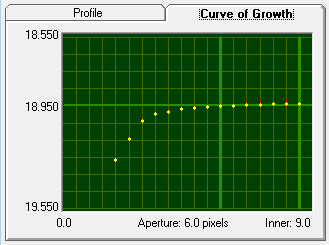
\includegraphics[scale=1.0]{Images/AsImages/SI/Sr1-Growth.PNG} \\ [0.2cm]
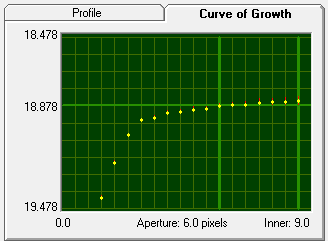
\includegraphics[scale=1.0]{Images/AsImages/SI/Sr3-Growth.PNG}
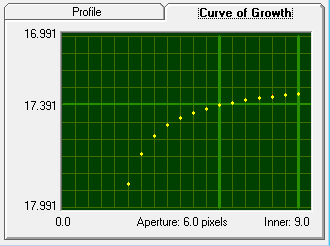
\includegraphics[scale=1.0]{Images/AsImages/SI/Sr2-Growth.PNG} \\ [0.2cm]
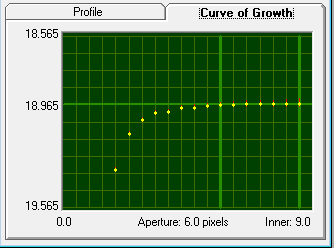
\includegraphics[scale=1.0]{Images/AsImages/SI/Sr4-Growth.PNG}
\end{multicols}
\caption{AIP4WIN image of the Messier 82 galaxy with the photometry tool 'Single-Image' depicting the photometric curves of growth of four stars surrounding the galaxy. Star 1 = top right, Star 2 = top right, Star 3 = bottom left and Star 4 = bottom right.}
\label{SI-Growth}
\end{figure}

AIP4Win determines the errorbars in \cref{SS-Growth} and \cref{SI-Growth} though small, they are a result of the a miscalculation of magnitude, as the star emits light flux that varies over the 60 second exposure time which thus the magnitude can change in values as the light flux fluctuates. \\

%---------------------------------------------------------------------------
%	SECTION 3
%---------------------------------------------------------------------------
\section{Multiple-Image Photometry}
\label{Section 3}

Multiple-Image photometry is used to measure raw instrumental or differential magnitudes from multiples images through an automated process (\cite{ImageProcessingTutorial}). By selecting a series of multiple images that have be taken over time, but first the images need to be calibrated first using two other files that set the zero the multiple image tool. Following this the target stars are selected  as shown in \cref{MI-Aperture} and multiple comparison stars to calculate around any atmospheric extinction present in front of the target star. By tracking mainly the target and first comparison star so when the software flicks through the series of images, it will track the two stars accurately due to the calibration earlier. The exported data collected is shown in \cref{MI Data} where the software extracted the magnitudes of each target star and comparison star. \\

\begin{figure}[H]
\centering
\begin{multicols}{2}
\begin{minipage}[H]{0.5\textwidth}
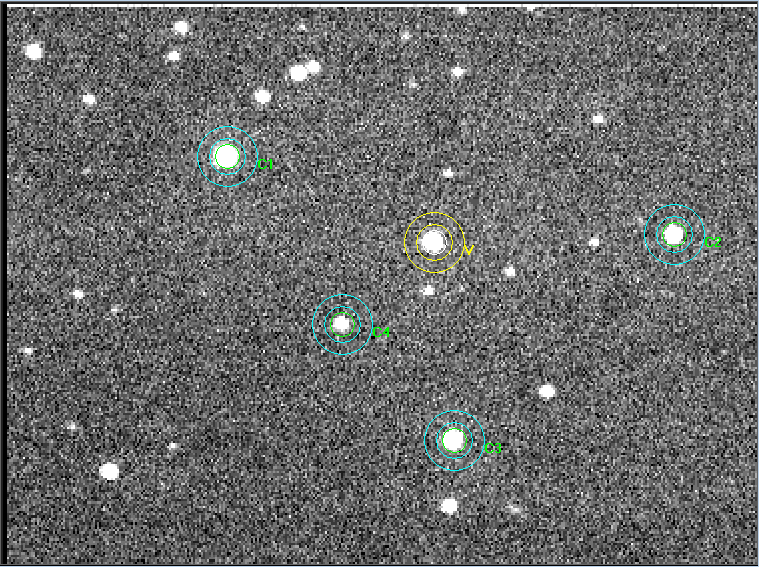
\includegraphics[scale=0.43]{Images/AsImages/MI/Sr1-Aperture.PNG} \\
\end{minipage}
\begin{minipage}[H]{0.5\textwidth}
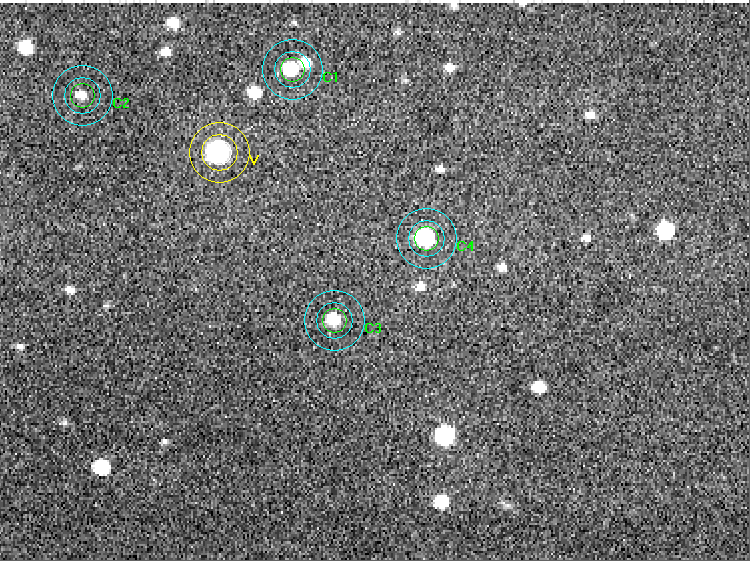
\includegraphics[scale=0.43]{Images/AsImages/MI/Sr3-Aperture.PNG}
\end{minipage}
\begin{minipage}[H]{0.5\textwidth}
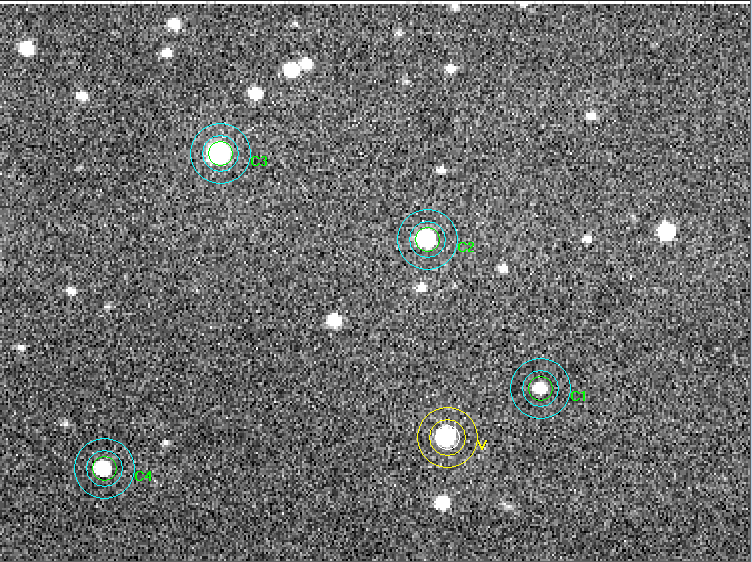
\includegraphics[scale=0.43]{Images/AsImages/MI/Sr2-Aperture.PNG} \\ 
\end{minipage}
\begin{minipage}[H]{0.5\textwidth}
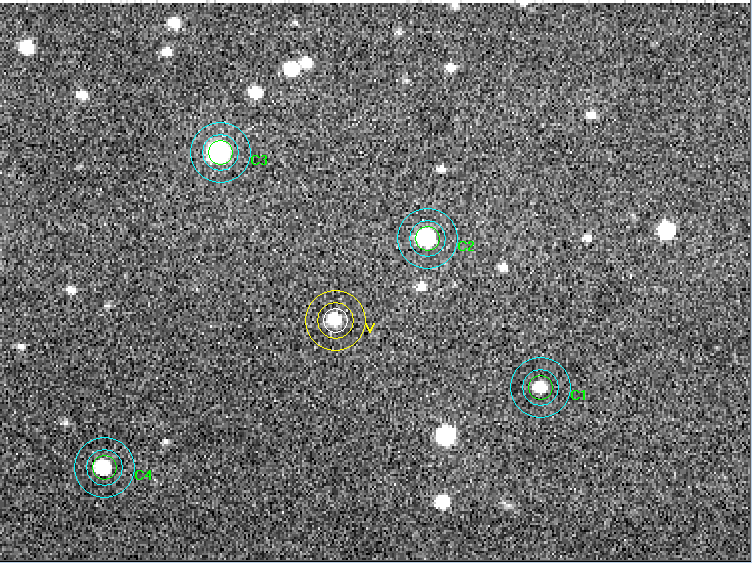
\includegraphics[scale=0.43]{Images/AsImages/MI/Sr4-Aperture.PNG}
\end{minipage}
\end{multicols}
\caption{AIP4WIN image of the Messier 82 galaxy with the photometry tool 'Multiple-Images' depicting the aperture, inner and outer anuli around each target star with 4 comparison stars for each target star for photometric measurements of four stars surrounding the galaxy. Star 1 = top right, Star 2 = top right, Star 3 = bottom left and Star 4 = bottom right.}
\label{MI-Aperture}
\end{figure}

\begin{table}[H]
\begin{center}
 \footnotesize
 \begin{tabular}{|c||c|c|c||c||c|c|}
 \hline
 \multicolumn{7}{|c|}{AIP4WIN Photometry settings for all four target single-image images} \\
 \hline \hline
 Target & Aperture & Inner Annulus & Outer Annulus & Sky Annulus & Integration & Zero  \\
 Star & Radius & Radius & Radius & Pixels & Time (s) & Point \\
 \hline \hline
 S1 & 6.0 & 9.0 & 15.0 & 234 & 60 & 25 \\
 \hline
 S2 & 6.0 & 11.0 & 15.0 & 231 & 60 & 25 \\
 \hline
 S3 & 6.0 & 11.0 & 15.0 & 131 & 60 & 25 \\
 \hline
 S4 & 6.0 & 9.0 & 15.0 & 231 & 60 & 25  \\
 \hline
 \end{tabular} \\ [0.5cm]
 \begin{tabular}{|c|c||c|c||c|c||c|c|}
 \hline
 \multicolumn{8}{|c|}{Photometric data collected of the four target single-image images} \\
 \hline \hline
 Star & Target & Star$_X$ & Star$_Y$ & ADU$_{Sky}$ & ADU$_{Star}$ & Magnitude & Sigma\\
 \hline \hline
 1&  Var & 215.002  &101.791  &         45.1197&    5871.51  & 19.073 &0.0296 \\
 1&  C1 & 111.480   &64.837     &     45.2025   &17950.15   &17.860 &0.0118\\
 1&  C2  &335.038   &98.486      &     44.8369   & 3365.82   &19.677& 0.0494\\
 1&  C3  &224.891  &186.961      &   44.8918    &7764.39  & 18.770 &0.0232\\
 1&  C4  &169.044  &137.099       &  44.6638   &1138.267  & 20.854 &0.1354\\
 1&Ens                     &  & & &                     30218.6   &17.294 &0.0119\\
 \hline \hline
 2& Var & 224.891 & 186.961  &  44.8918 &   7764.39  & 18.770 &0.0232\\
  2 & C1 & 271.700  &166.176   &      44.5127 &   949.267 &  21.051& 0.1654\\
  2& C2  &215.002  &101.791    &       45.1197  &  5871.51 &  19.073& 0.0296\\
  2& C3  &111.480   &64.837  & 45.2025  & 17950.15  & 17.860 &0.0118\\
  2& C4   &53.397  &200.481   &  44.2076  &  2787.86  & 19.882 &0.0587\\
  2&Ens                          &     & & &              27558.8  & 17.394 &0.0129\\
 \hline \hline
 3& Var & 224.891 & 186.961 &    44.8918  &  7764.39   &18.770 &0.0232 \\
 3&  C1&  271.700 & 166.176  &  44.5127   & 949.267   &21.051& 0.1654\\
  3& C2&  215.002 & 101.791  &  45.1197   & 5871.51   &19.073 &0.0296\\
  3& C3 & 111.480 &  64.837   &  45.2025   &17950.15  & 17.860& 0.0118\\
  3& C4 &  53.397 & 200.481  &   44.2076  &  2787.86 &  19.882 &0.0587\\
  3&Ens                        &  & & &                  27558.8 &  17.394& 0.0129\\
 \hline \hline
  4&Var & 224.891 & 186.961   &   44.8918   & 7764.39  & 18.770 &0.0232\\
  4&  C1  &271.700 & 166.176   &   44.5127  &  949.267 &  21.051& 0.1654\\
   4& C2  &215.002 & 101.791  &  45.1197   & 5871.51   &19.073& 0.0296\\
   4& C3  &111.480  & 64.837   &  45.2025   &17950.15  & 17.860 &0.0118\\
   4& C4  & 53.397 & 200.481   &  44.2076  &  2787.86 &  19.882& 0.0587\\
  4& Ens                     &   & & &                    27558.8  & 17.394 & 0.0129\\
 \hline 
 \end{tabular} \\[0.5cm]
 \begin{tabular}{|c||c|c|c|}
 \hline
 \multicolumn{4}{|c|}{Magnitudes for all four target single-image images} \\
 \hline 
 Star & (V-C1) \& Sigma & (C2-C1) \& Sigma & (V-Ens) \& Sigma\\
 \hline \hline
 1 & 1.213 $\pm$ 0.032 &  1.817 $\pm$ 0.051 &  1.779 $\pm$ 0.0132 \\
 \hline
 2 & -2.282 $\pm$ 0.0167 &  -1.978 $\pm$ 0.168 &  1.375 $\pm$ 0.027 \\
 \hline
 3 & -2.282 $\pm$ 0.167 &  -1.978 $\pm$ 0.168 &  1.375 $\pm$ 0.027 \\
 \hline
 4 & -2.282 $\pm$ 0.167 &  -1.978 $\pm$ 0.0168 &  1.375 $\pm$ 0.072 \\
 \hline
 \end{tabular} \\
 \caption{AIP4WIN settings and photometry data of the 4 target 'multiple-image' stars.}
 \label{MI Data}
\end{center}
\end{table} 

As in \cref{SubSection 2b}, the software subtracts the first comparison star from the target star to give a differential magnitude. Below in \cref{MI-Profile}, the profile of the difference in magnitude allows us to see how the differential magnitude differs in each images, the errorbars are extreme of three of them at the star has moved significantly over the time duration of the series of images.

\begin{figure}[H]
\centering
\begin{multicols}{2}
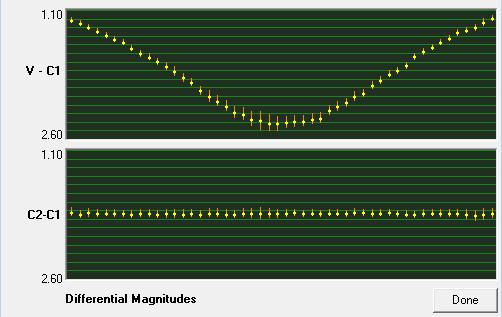
\includegraphics[scale=0.65]{Images/AsImages/MI/Sr1-Profile.PNG} \\ [0.2cm]
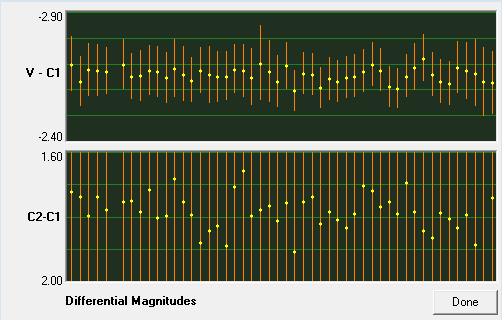
\includegraphics[scale=0.65]{Images/AsImages/MI/Sr3-Profile.PNG}
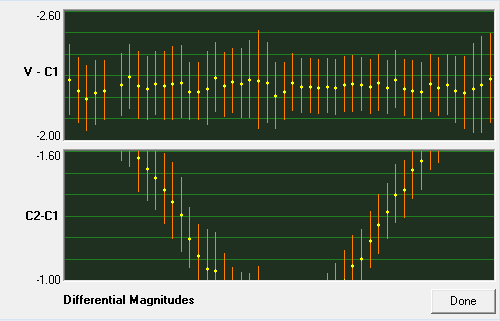
\includegraphics[scale=0.65]{Images/AsImages/MI/Sr2-Profile.PNG} \\ [0.2cm]
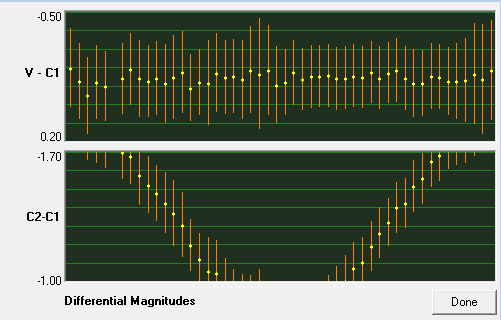
\includegraphics[scale=0.65]{Images/AsImages/MI/Sr4-Profile.PNG}
\end{multicols}
\caption{AIP4WIN image of the target star system with the photometry tool 'Multiple-Images' depicting the photometric curves of growth of four stars surrounding the galaxy. Star 1 = top right, Star 2 = top right, Star 3 = bottom left and Star 4 = bottom right.}
\label{MI-Profile}
\end{figure}

%---------------------------------------------------------------------------
%	SECTION 4
%---------------------------------------------------------------------------
\section{The Carina Nebula}
\label{Section 4}

\begin{figure}[H]
\centering
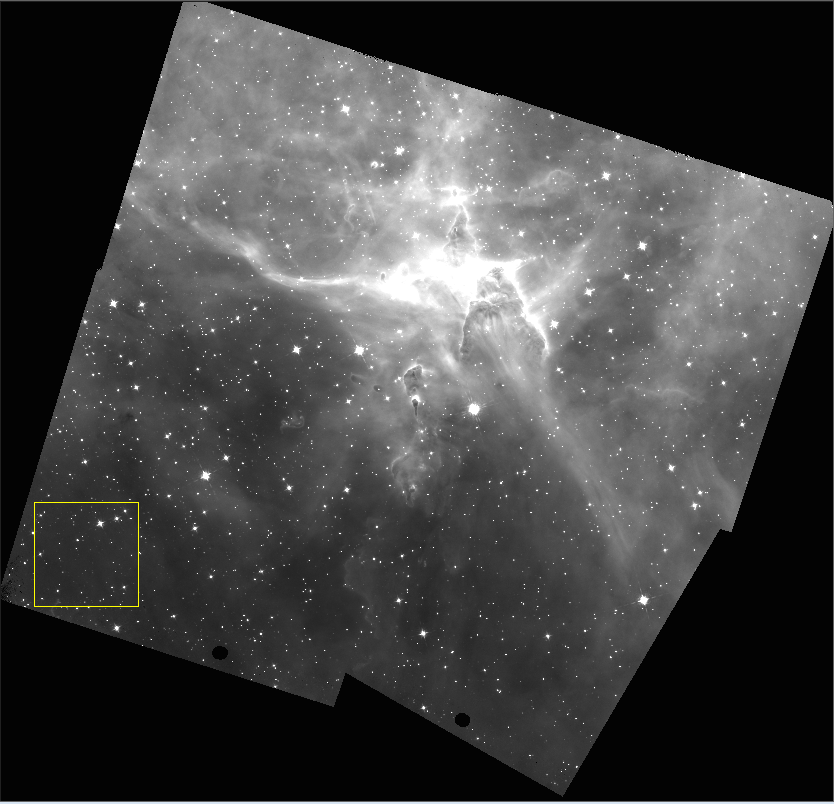
\includegraphics[scale=0.6]{Images/AsImages/CN/Crop.PNG}
\caption{An infrared image of the Carina Nebula source from (\cite{CarNeb}).}
\label{Carina}
\end{figure}

Sourcing a infrared image (\cref{Carina}) of the Carina Nebula (\cite{CarNeb}) and cropping a square section of the image at 40 arcseconds across each side allows for a small photometric measurement to take place, though the software only allows for pixels measurements, not arcseconds to be entered so converting 40 arcseconds into pixels:

\begin{equation}
\dfrac{0.128"}{Pixel} \rightarrow \dfrac{0.128"}{40"} = 312.5 Pixels
\end{equation} \\

\begin{figure}[H]
\centering
\begin{multicols}{2}
\begin{minipage}[H]{0.5\textwidth}
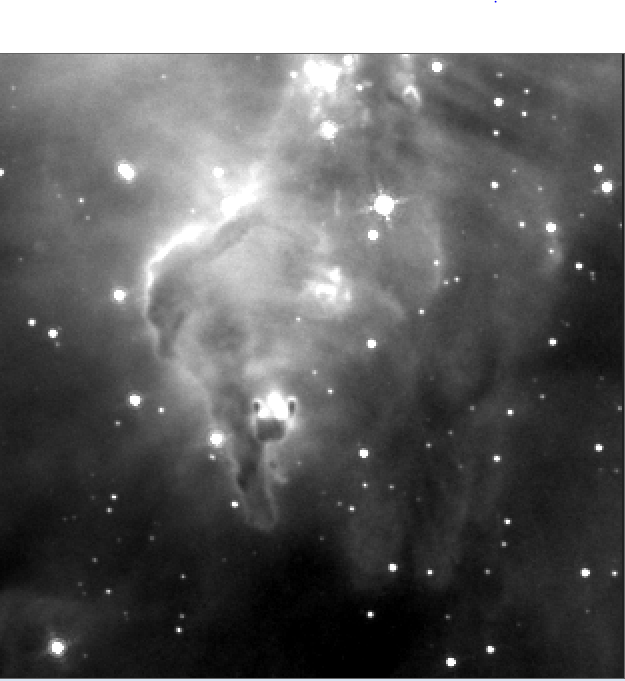
\includegraphics[scale=0.475]{Images/AsImages/CN/Stars.PNG}
\end{minipage}
\begin{minipage}[H]{0.5\textwidth}
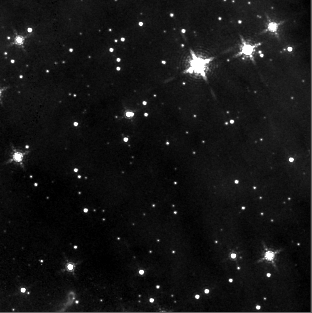
\includegraphics[scale=0.95]{Images/AsImages/CN/darksky.PNG}
\end{minipage}
\end{multicols}
\caption{Two cropped images of the nebula + sky and the sky background.}
\label{CN}
\end{figure}

Selecting an area of the \cref{Carina} where there is plenty of light from the nebula with a selection of star is necessary to extract as much clear data so to estimate the instrumental magnitude of the nebula in the cropped area. Using the cropped image of the nebula + sky shown in \cref{CN}, using the pixel tool on multiple areas of the nebula gives the mean total of pixel counts over a area containing a number of pixels and their individual standard errors shown in \cref{CN-Sky Data}. The same is done to a 40 arcseconds cropped section of dark sky background which copies the amount of stars in the original cropped image but has a majority of dark sky illustrated in \cref{CN} where the data collected is display in \cref{CN-Sky Data}. \\

\begin{table}[H]
\begin{center}
 \footnotesize
 \begin{tabular}{|c|c|c||c|c|c|}
 \hline
 \multicolumn{6}{|c|}{Values of light flux for the nebula \& sky of the Carina Nebula} \\
 \hline
 \textbf{Mean} & \textbf{Pixels} & \textbf{Std Dev} & \textbf{Mean} & \textbf{Pixels} & \textbf{Std Dev}\\
 \hline \hline
 2.49382 & 349 & 0.049855	 & 0.893753 & 641 & 0.02178 \\
 \hline
 1.95734 & 725 & 0.151801	& 0.736952 & 457 & 0.02077 \\
 \hline
 2.57294 & 1403 & 0.036983 & 0.9239792 & 1033 & 0.157065 \\
 \hline
 2.74983 & 277 & 0.033442	 & 0.978278 & 545 & 0.027846 \\
 \hline
 2.48937	& 657 & 0.045167	&	0.867642&	1281	&0.022931 \\
 \hline
 2.43827	&1425	& 0.068683&		0.907267&	401&	0.017125\\
 \hline
 2.34643	&1389	&0.110985	&	0.826468&	741	&0.020146\\
 \hline
 2.04743&	805&	0.037392	&	0.862156&	697&	0.023058\\
 \hline
 2.04722&	1041&	0.083214	&	0.926473&	1033&	0.031044\\
 \hline
2.00573&	697	&0.057807	&	0.975374&	1289&	0.037345\\
 \hline
 1.84873&	473&	0.058754	&	0.974485&	1209&	0.022581\\
 \hline
 2.46837&	965&	0.039759	&	0.8529552&	275&	0.019286\\
 \hline
 2.85937&	811	&0.036607	&	0.826752&	517&	0.021443\\
 \hline
 2.35838&	965	&0.129077	&	0.9782558&	1473&	0.021104\\
 \hline
 2.48284&	933	&0.109176	&	0.974245&	1245&	0.030159\\
 \hline
 2.58492&	497	&0.052405	&	0.878278&	697&	0.030214\\
 \hline
 1.88623&	505	&0.029356	&	0.8264654&	741&	0.028294\\
 \hline
 2.46245&	593	&0.050433	&	0.865254&	609&	0.019732\\
 \hline
 2.89628&	1549	&0.118608	&	0.988724&	1177&	0.029515\\
 \hline
 3.17362&	1900	&0.101	&	0.998762&	1137&	0.024223\\
 \hline
 2.97266&	1669	&0.07851	&	0.799624&	593&	0.021649\\
 \hline \hline
 \textbf{2.435344286}	& \textbf{934.6666667} &	\textbf{0.070429238}	&	\textbf{0.898197267} & \textbf{ 847.1904762} & \textbf{0.030824286}\\
 \hline
 \end{tabular} \\ [0.5cm]
 \begin{tabular}{|c||c|c|c|c|c||c|}
 \hline
 \multicolumn{7}{|c|}{Results of the flux and magnitude of the Nebula only} \\
 \hline \hline
   & Neb - Sky & Pixels in Area & Total Nebula & Exp.Time (s) & Flux & Magnitude \\ 
 \hline
 Values & 1.537 & 98656.25 & 151649.161 & 699.232 & 216.8795 & 19.159454 \\
 \hline
 Error & 0.03960495 & 98 656.25 & 3907.27605 & 699.232 & $\pm$5.58795 & $\pm$2.8 \\ 
 \hline
 \end{tabular} \\ 
 \caption{Tabular results of the Nebula - Sky background calculations.}
 \label{CN-Sky Data}
\end{center}
\end{table} 

To obtain a instrumental magnitude of the Carina Nebula its necessary to obtain a magnitude of the nebula without the sky background interference, so in \cref{CN-Sky Data} by taking an average mean and standard deviation error, the sky background data will be subtracted from the nebula + sky data. The nebula only value will then multiplied by the amount of pixels in the cropped image which is 98656.25 pixels (312.5 multiplied by itself), this gives a total nebula value of 151649.161. To calculate the amount of flux in the nebula, the total nebula count is divided by the exposure time, then using the flux to calculate the instrumental magnitude. \\

\begin{equation}
Flux_N = \dfrac{151649.161}{699.232483} = 216.879456 \pm 5.588
\end{equation} \\

\begin{equation}
M_I = -2.5 \times log(216.879456) + 25 = 19.159454 Mag \pm 2.8 Mag
\end{equation}

To calculate the nebula + stars instrumental magnitude, the same cropped image of the nebula is used but using the single star tool to measure their individual magnitudes. But this only gives the magnitude of the star not with the nebula, so by measuring the magnitudes of the most prominent stars in nebula image of \cref{CN} to which the data is displayed in \cref{CN-Stars Data}. 

\begin{table}[H]
\begin{center}
 \footnotesize
 \begin{tabular}{|c|c|c|c||c||c|c|}
 \hline
 \multicolumn{7}{|c|}{Values of light flux for the stars of the Carina Nebula} \\
 \hline
 \textbf{Star} & \textbf{X Pos} & \textbf{Y Pos} & \textbf{Magnitude} & \textbf{Error} & \textbf{Flux} & \textbf{Corrected Flux}\\
 \hline \hline
 1&191.559 & 74.97&24.551	&0.136	&	1.512167849	&149184.8093 \\
 \hline
 2&62.621&	58.314&	25.459&	0.312	&	0.655239394	&64643.46147 \\
 \hline
 3&59.165&	120.128&	26.131&	0.569	&	0.352858026	&34811.64961 \\
 \hline
 4&67.01&	172.512&	26.219&	0.599	&	0.325386852	&32101.4466 \\
 \hline
 5&107.671&	191.974&	25.736&	0.39	&	0.507691626	&50086.95197 \\ 
 \hline
 6&181.413&	199.205&	27.344&	1.738	&	0.115451612	&11390.02307\\ 
 \hline
 7&185.367&	144.403&	27.403&	1.848	&	0.10934527	&10787.59426 \\
 \hline
 8&163.921&	37.429&	25.463&	0.308	&	0.652829844	&64405.74431 \\
 \hline
 9&275.028&	86.255&	26.987&	1.232	&	0.160398388	&15824.30349 \\ 
 \hline
 10&275.91&	143.523&	28.358&	4.361	&	0.045373262	&4476.355849 \\
 \hline \hline
 & & \textbf{263.651}	& \textbf {11.493}	& 	\textbf{4.436742122}	& \textbf{437712.34} \\
 \hline
 \end{tabular} \\ [0.5cm]
 \begin{tabular}{|c||c|c|c|c|c||c|}
 \hline
 \multicolumn{7}{|c|}{Results of the flux and magnitude of the Nebula only} \\
 \hline \hline
   & Neb - Sky & Pixels in Area & Avg. Neb & Exp.Time (s) & Flux & Magnitude \\ 
 \hline
 Values & 1.537 & 98656.25 & 151649.161 & 699.232 & 216.8795 & 19.159454 \\
 \hline
 Error & 0.03960495 & 98 656.25 & 3907.27605 & 699.232 & $\pm$5.58795 & $\pm$ 0.5 Mag \\ 
 \hline
 \end{tabular} \\ 
 \caption{Tabular results of the Star + Nebula calculations.}
 \label{CN-Stars Data}
\end{center}
\end{table} 

\begin{figure}[H]
\centering
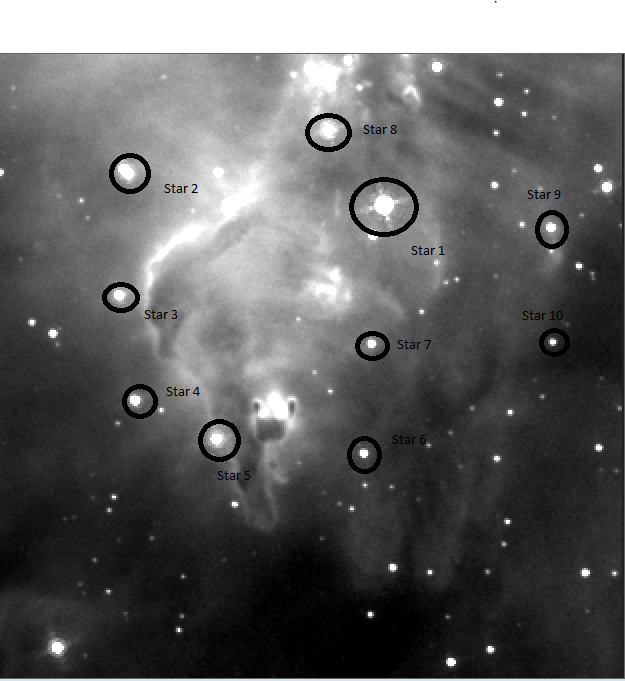
\includegraphics[scale=0.55]{Images/AsImages/CN/StarsE.PNG}
\caption{The Stars as in relation to \cref{CN-Stars Data}.}
\label{CarinaE}
\end{figure}

The magnitudes are calculated into flux and total using:

\begin{equation}
Flux_S = 10^{(Magnitude-25)/-2.5} = 4.4367
\end{equation} \\

The flux needs to be transformed into counts where it can be related to the pixel area of the image and the exposure time and recalculated into flux:

\begin{equation}
Flux_S = \dfrac{(4.4367 \times 699.232482)\times 98656.25}{699.232483} = 437712.34
\end{equation} \\

Adding the flux that was calculated for the nebula only to this flux value and finding the instrumental magnitude again but this time for the nebula + stars:

\begin{equation}
M_I = -2.5 \times log(216.879456 + 437712.34) + 25 = 10.8965 Mag \pm 0.52 Mag
\end{equation} \\

This final value for the instrumental magnitude makes sense as the more negative the magnitude, the brighter it is and comparing it to the nebula only magnitude of 19 Mag and as the nebula + stars equals to be 10 which is logical as it contains measurements of stars which are brighter than the nebula itself.  \\

%---------------------------------------------------------------------------
\addcontentsline{toc}{section}{References}
\bibliographystyle{plain}
\bibliography{mybib.bib}
\end{document}